
% Say what the application is
In this analysis dijet tracks are being clustered, using a method known as {\it hierarchical clustering}, according to 
their $L_{xy}^\text{exp}$ as described in Section \ref{subsec:Clusters}.

Hierarchical clustering connects elements of an unclustered set using a similarity (linkage) criterion,
as shown schematically in Figure \ref{fig:dendrogram}.
\begin{figure}[htbp]
\centering
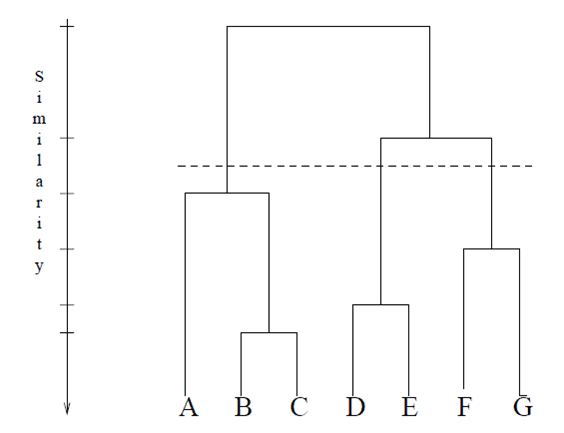
\includegraphics[width=0.5\textwidth]{plots/dendrogram2.png}
% correct the plot
\caption{Dendrogram presenting hierarchical clustering. \label{fig:dendrogram}}
\end{figure}

 Initially each element is its own cluster (A-G). Each of the next steps merges 
 two most similar clusters into one.
In case of clustering numbers the similarity criterion is the minimal distance 
between clusters. For clusters A and B the similarity is obtained as follows:

\begin{equation}
\min \{\, d(x,y) : x \in \mathcal{A},\, y \in \mathcal{B} \,\}, \hspace{5pt} d(x,y)=|x-y| 
\label{eqn:linkage}
\end{equation}

where $\mathcal{A}$ and $\mathcal{B}$ are already existing clusters.
 As presented in Figure \ref{fig:dendrogram} the first step connects clusters B and C, the second step connects clusters D and E, etc.
The procedure repeats until the similarity criterion is no longer satisfied. In Figure \ref{fig:dendrogram} the minimal similarity criterion is 
schematically presented as a horizontal
dashed line. The clustering procedure results in two clusters: ABC and DEFG. In the dijet analysis we cluster tracks according to 
their $L_{xy}^\text{exp}$ only, if the minimal distance between the clusters (Eqn. \ref{eqn:linkage}) does not exceed 15\% of the secondary vertex $L_{xy}$.

